\section*{Задание}
\addcontentsline{toc}{section}{Задание}

Разработать программу "Виндоуз мобиле", функционирующую в рамках пяти процессов
(отец и 4 сына). Процесс-отец, имитируя работу ядра ОС, порождает 4
процесса-сына. Каждый сын регистрирует функцию-обработчик сигнала \texttt{SIGUSR1} и
переходит в состояние ожидания посредством pause(). Процесс-отец читает со
стандартного ввода цифру в диапазоне 0 \ldots ~3 (имитация касания какой-либо иконки
на экране планшета/смартфона) и посылает сигнал \texttt{SIGUSR1} соответствующему
процессу-сыну. Разбуженный сигналом процесс считывает со стандартного ввода одну
строку символов, преобразует её соответственно своей функциональности, выводит
результат в стандартный вывод и возвращается в состояние сна. Процессы-сыновья
имеют следующие функциональности:
\begin{itemize}
    \item 0 - смена "регистра" всех символов;
    \item 1 - инвертирование строки - первый символ становится последним и т.д.;
    \item 2 - обмен соседних символов - нечетный становится на место четного и наоборот;
    \item 3 - перевод в КОИ-8 - установление в 1 старшего (8-ого) бита каждого символа.
\end{itemize}
Для чтения цифры с клавиатуры в процессе-отце использовать неканонический режим.

\newpage

\section*{Описание структуры программы}
\addcontentsline{toc}{section}{Описание структуры программы}

В реализации данной программы было использовано 5 процессов: 1 родительский и 4 дочерних.
Родительский процесс считывает ввод пользователя, обрабатывает его и на его
основе запускает необходимый дочерний процесс, используя сигнал \texttt{SIGUSR1}.

Дочерний сигнал считывает строку символов, выполняет характерное действие над
ней и заного активирует родительский процесс.

Этот цикл повторяется, пока не будет нажата комбинация клавиш \^{}C, после чего
произойдет поочередное завершение всех дочерних процессов и выход из программы

Более подробная схема использования сигналов в программе приведена на рис. \ref{fig:signals}

\begin{figure}[h]
    \centering
    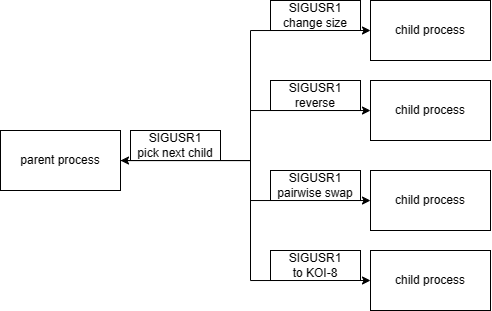
\includegraphics[width=0.6\linewidth]{images/lab1_signals.drawio.png}
    \caption{Схема распространения сигналов}
    \label{fig:signals}
\end{figure}

\newpage

\section*{Блок-схема программы}
\addcontentsline{toc}{section}{Блок-схема программы}

% \begin{figure}[h]
%     \centering
%     \includegraphics[width=0.6\linewidth]{images/flowchart.png}
%     \caption{Блок-схема программы}
%     \label{fig:flowchart}
% \end{figure}

\newpage

\section*{Результат работы}
\addcontentsline{toc}{section}{Результат работы}

Тут должны быть скрин-шоты, чтобы показать, что программы работает
динамически.

Ниже показан запуск программы. Таймер работает изначально с интервалом 1.
После было нажато сочетание клавиш \texttt{CTRL-C}, \texttt{Enter}
\texttt{CTRL-D}.

\newpage

\appendix

\section*{Приложение}
\section*{Текст программы}
\addcontentsline{toc}{section}{Текст программы}

\begin{verbatim}
#include <unistd.h>
#include <stdlib.h>
#include <signal.h>

int G_TIMER_DURATION = 1;
void change_timer_duration(int code)
{
    if (G_TIMER_DURATION == 1)
        G_TIMER_DURATION = 3;
    else
        G_TIMER_DURATION = 1;
}

void foo(int code) {}

/* дочерний процесс */
void child_process()
{
    /*child*/
    char msg[1];
    signal(SIGUSR1, change_timer_duration);
    signal(SIGUSR2, exit);
	/*
	создаем пустой обработчик, который нужен для работы alarm, pause
	*/
    signal(SIGALRM, foo);
    while (1)
    {
        /*sleep(G_TIMER_DURATION);*/
        alarm(G_TIMER_DURATION);
        pause();
        *msg = G_TIMER_DURATION + '0';
        write(1, msg, 1);
    }
}

/* родительский процесс */
void parent_process(int child)
{
    char ch[1];
    int read_size;
    while (1)
    {
        read_size = read(0, ch, 1);
        if (read_size == 0)
        {
            /*
            обработка Ctrl-d
            отправка сигнала завершения программы
            */
            kill(child, SIGUSR2);
            exit(0);
        }
        /* обработка Enter и отправка сигнала смены инетрвала*/
        if (*ch == '\n')
            kill(child, SIGUSR1);
    }
}

int main()
{
    /* игнорируем ненужные сигналы */
    signal(SIGINT, SIG_IGN);
    signal(SIGQUIT, SIG_IGN);
    pid_t child = fork();
    /* обработка ошибок */
    if (child == -1)
    {
        write(2, "We can create a process\n", 24);
        exit(-1);
    }
    if (child == 0)
        child_process();
    else
        parent_process(child);
}
\end{verbatim}
